\section{Background}
\begin{itemize}
    \item Husk rød tråd.
    \item Vær generisk.
    \item Bare inkluder konsept som blir relevante senere, eller som er brukt i nødvendige antagelser.
    \item many of the concepts explained in this chapter were also explained in [TODO: fordypningsprosjekt].
    \item The goal of this chapter is to explain all the concepts neccessary to understand how the trajeoctyr planning algorithm works.
    Additionally, it should grant an understanding as to why the algorithm ended up the way it is.
\end{itemize}

\subsection{Target Ship prediction}
--------- Genereal thoughts --------------------------
\begin{itemize}
    \item Gjenfortelling fra fordypningsprosjekt, da kalt traffic pattern
    \item Fant en annen artikkel fra Kina som skrev om nogenlunde det samme, \gls{AIS} data -\> prediksjon
    \item Skiller seg fra fordypningsprosjekt fordi det er egentlig ikke traffic pattern som er den viktige antagelsen,
    Det er heller viktig at vi antar det finnes en måte å gjette/vite hvor andre båter vil være fremover i tid.
    \item Andre metoder for target ship prediction kan være f.eks utvidelse av \gls{AIS} som 
    inkluderer autonav data for de neste 5 minuttene eller noe lignende.
\end{itemize}
---------- /General Thoughts--------------------------- 
\begin{itemize}
    \item Naval navigation is an 'active' task, always looking out for obstacles and making sure the way forward is clear.
    \item There are no lanes, instead proper conduct is dictated by \gls{COLREGs}, the rules are laid out so that different situations
    have different rules
    \item Knowing which situation you are in is half the battle, therefor the ability to predict and estiamte how encounters will happen
    is a powerful tool. Human navigators do this by experience.
    \item Autonomous vessels could also predict by experience, that would be the machine learning approach. \gls{AIS} can already provide training data.
    \item But it could be easier than that, what if \gls{AIS} data packets were expanded to send out autonav data for where a vessel intends to traverse.
    The assumption here is that vessels using autonav will correct their course when spotting a conflict. Vessels not using autonav would still be able to observe
    the indended path of other vessels and adjust their plans 'manually'.
    \item Relying on fully predicting the transit of a target vessel is fragile, relying on a few known waypoints would be much more robust.
    \item In the end the best solution would be if all vessels could fully communicate their intended path either peer to peer or through
    a centralized system. Solving conflicting paths would be done on a higher level than individual vessel.
\end{itemize}

\begin{figure}
    \centering
    \label{FIG: AIS lanes}
    \includegraphics[width=\textwidth]{Images/AISLanes.jpg}
    \caption{TODO: Skriv. AIS data can show common transit routes. Image courtesy of Olex AS}
\end{figure}


\subsection{Vessel modelling}
--------- Genereal thoughts --------------------------

Jeg tenker det er best å skrive om modellering i sammenheng med hvordan trajectory planning problemet blir satt opp i MATLAB med CasADi.
\begin{itemize}
    \item Kinematics \& Kinetics -\> Begge brukes i CasADi setup
    %\item Munk moment -> Potensielt relevant hvis jeg skriver om modellerings problemer
    \item Her kan det også skrives om de spesifike tallverdiene som blir brukt i Masse, coriolis og dempnings -matrisene.
    de er spesifike til Milliampere, funnet gjennom en rekke forsøk utfort av Anders Pedersen.
\end{itemize}
---------- /General Thoughts--------------------------- 

\begin{figure}
    \centering
    \label{FIG: Ship DOF}
    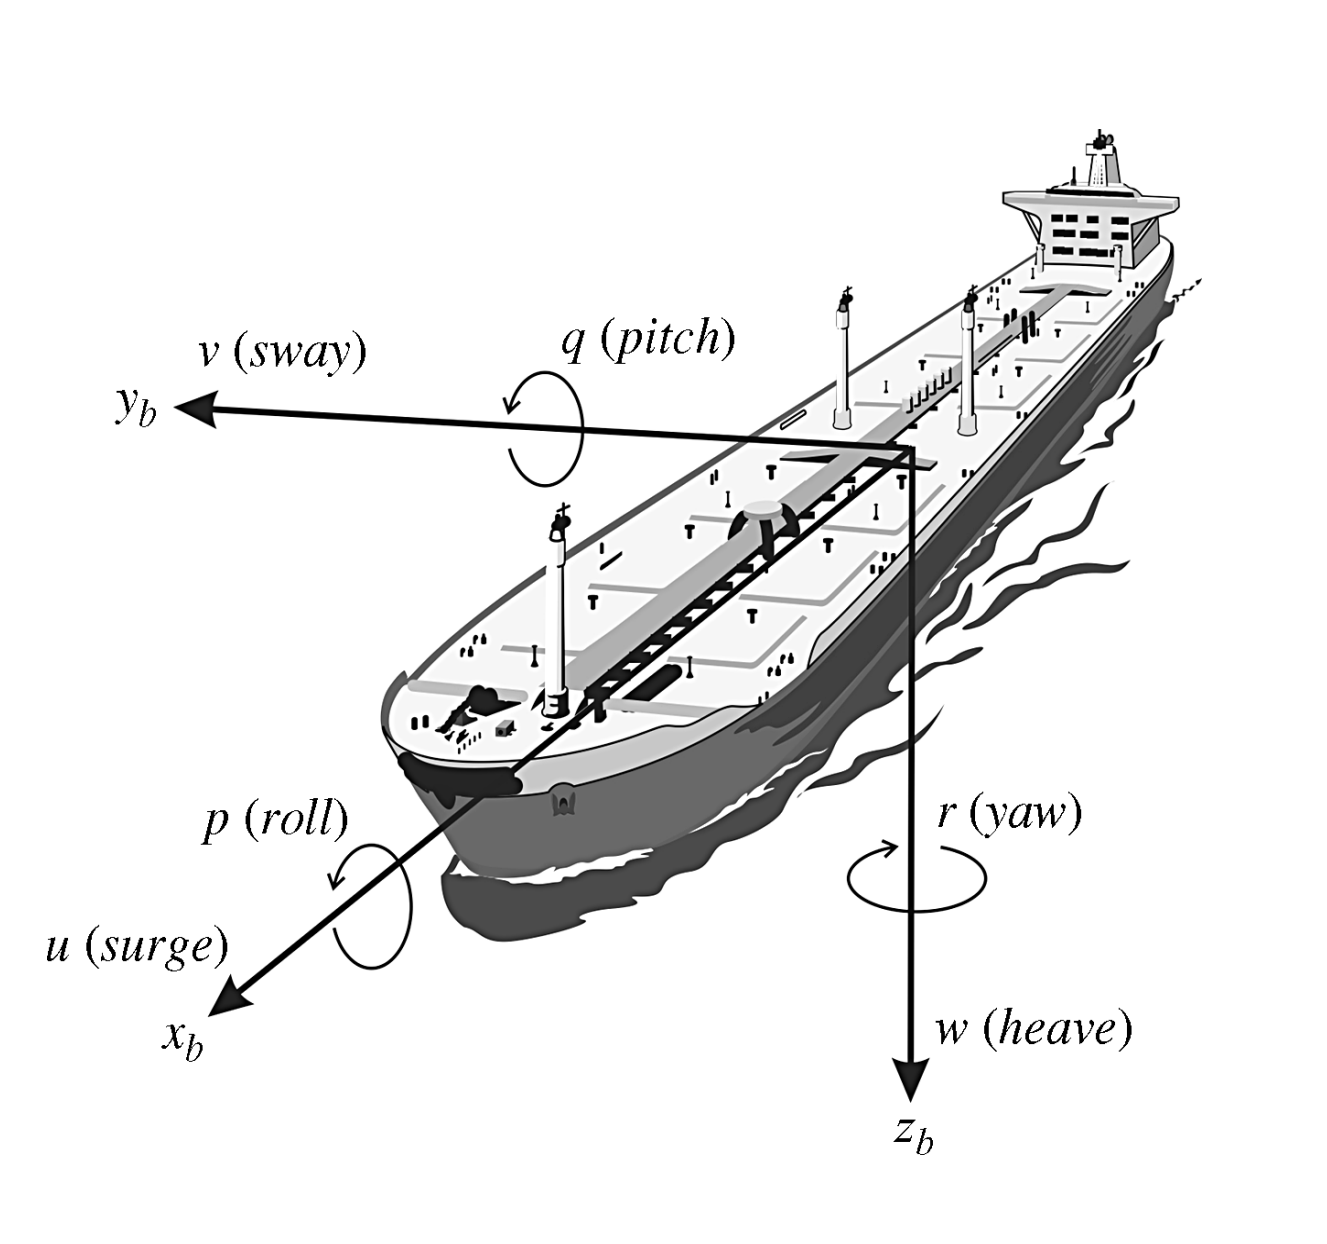
\includegraphics[height=0.35\textheight]{Images/SHIPDOF_FOSSEN.png}
    \caption{A ships 6 degrees of Freedom, from \cite{fossen2011handbook}}
\end{figure}

\begin{itemize}
    \item 3 \gls{DOF} non-linear model with thurster dynamics, very common for designing control systems.
    \item The numerical values for the model will vary based on ship, and the complexity of the model change based on usage and the degrees of freedom included.
    \item The model used in this paper is based on Fossen's meneuvering theory with 3 degrees of freedom and no disturbances.
\end{itemize}

\begin{equation}
    \bm{\dot{\eta}} = \textbf{R}(\psi)\bm{\nu}    
\end{equation}
\begin{equation}
    \textbf{M}\bm{\dot{\nu}} + \textbf{C}(\bm{\nu})\bm{\nu} + \textbf{D}(\bm{\nu})\bm{\nu} = \bm{\tau}
\end{equation}
\begin{equation}
    \textbf{R}(\psi) = \begin{bmatrix}
                        cos\psi &   -sin\psi & 0\\[-5pt]
                        sin\psi & cos\psi    & 0\\[-5pt]
                        0       &   0        & 1
                        \end{bmatrix}
\end{equation}
\begin{equation}
    \bm{\eta} = \begin{bmatrix}
                x   &    y  &    \psi
                \end{bmatrix}^T
\end{equation}
\begin{equation}
    \bm{\nu} = \begin{bmatrix}
                 u   &   v  &    r
                \end{bmatrix}^T
\end{equation}
\begin{equation}
    \bm{\tau} = \begin{bmatrix}
                F_{X}   &   F_{Y}  &   F_{N}
                \end{bmatrix}^T
\end{equation}

\begin{itemize}
    \item $\eta$ is defined in the \gls{NED} reference frame, $\nu$ is defined in BODY frame, briefly explain what that means.
    \item The M and C matrices are a combination of Rigid body and hydrodynamic added mass matrices
    \item Fully computing the M and C matrices is a lot of work, for milliampere the work has already been conducted
    by Andreas Pedersen.
    \item If the model values are to be found through experiementation it's senseless to seperate Rigid body and hydrodynamic added mass.
    The matrices then become:
\end{itemize}

\begin{equation}
    \textbf{M} = \begin{bmatrix}
                m11 &   m12 &   m13\\[-5pt]
                m12 &   m22 &   m23\\[-5pt]
                m31 &   m32 &   m33
                 \end{bmatrix}
\end{equation}

\begin{equation}
    \textbf{C}(\bm{\nu}) =  \begin{bmatrix}
        0             &     0       &   c13(\bm{\nu})\\[-5pt]
        0             &     0       &   c23(\bm{\nu})\\[-5pt]
        c31(\bm{\nu}) &c32(\bm{\nu})&   0
                            \end{bmatrix}    
\end{equation}

\begin{equation}
    \textbf{D}(\bm{\nu}) =  \begin{bmatrix}
        d11(\bm{\nu}) &     0       &   0\\[-5pt]
        0             &d22(\bm{\nu})&d23(\bm{\nu})\\[-5pt]
        0             &d32(\bm{\nu})&d33(\bm{\nu})
                            \end{bmatrix}       
\end{equation}

\begin{itemize}
    \item The D matrix can sometimes be a bit of a nuisance, a simplified D matrix can be employed to make
    the model more computationally efficient, at the cost of accuracy.
\end{itemize}

\begin{equation}
    \textbf{D}(\bm{\nu}) = \begin{bmatrix}
                            d11 &   0   &   0\\[-5pt]
                            0   &   d22 &   0\\[-5pt]
                            0   &   0   &   d33
                            \end{bmatrix}
\end{equation}

\subsection{Trajectory Planning}
--------- Genereal thoughts --------------------------
\begin{itemize}
    \item How to get from A to B.
    \item Multiple methods, all with pros and cons, skriv liten oversikt.
    \subitem LOS, OCP, Machine Learning, osv.
    \subitem Kanskje ikke så veldig viktig å snakke om andre metoder enn OCP.  
    \item Important factors to consider:
    \subitem Time horizon / length of planning period.
    \subitem Trajectory safety with respect to ship capabilities.
    \subitem \gls{COLREGs} compliance with respect to expected behaviour.
    \subitem osv.
    \item Litt dypere inn i numerisk optimalisering og MPC, og LOS ettersom det kommer til å bli brukt igjen senere.
   % \item Først oversikt, deretter enten nytt kapittel eller delkapittel om 
   % den spesifikke metoden jeg skal bruke, forklar numerisk optimalisering, MPC, LOS guidance, hvordan alt kombineres til å bli min algoritme, in theory.
\end{itemize}
--------- /Genereal thoughts --------------------------
\begin{subequations}
    \label{eq:OCP description}
\begin{align}
    \textrm{Minimize} \quad & \textbf{F}(\boldsymbol{\eta}(t), \textbf{u}(t)) \label{eq:OCP-a} \\ 
    \textrm{subject to} \quad & \dot{\boldsymbol{\eta}}(t) = \textbf{L}(\boldsymbol{\eta}(t), \textbf{u}(t)) \label{eq:OCP-b} \\
    \quad & \textbf{h}(\boldsymbol{\eta}(t), \textbf{u}(t)) \leq \textbf{0} \label{eq:OCP-c}\\
    \quad & \boldsymbol{\eta}(t_0) = \boldsymbol{\eta}_0 \label{eq:OCP-d}
\end{align}
\end{subequations}
(TODO: REWRITE THIS, SOME PARTS MAKE LITTLE SENSE)\\
where $\textbf{F}$ is the objective function, $\boldsymbol{\eta}(t)$ is the position and attitude trajectory of the vehicle, $\textbf{u}(t)$
is the control input trajectory and $\textbf{L}$ is the kinematic model of the vehicle. Though the OCP can be solved
the way it is set up in (\ref{eq:OCP description}) it is more pratical to discretize it into a ( \gls{NLP}).
With a method called direct multiple shooting, both state and control input are defined as decision variables, the  \gls{NLP} with
$N$ control intervals is:

\begin{figure}
    \label{FIG: Shooting Gaps}
    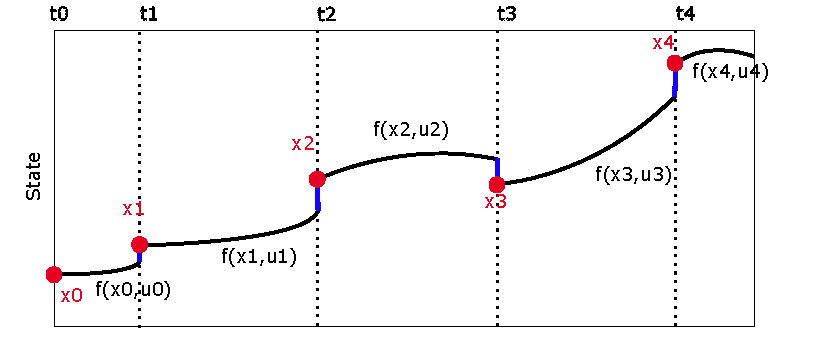
\includegraphics[width=\textwidth]{Images/MultipleShooting.pdf}
    \caption{A physically feasible trajectory is formed by "pinching" the shooting gaps so they close. Reproduction of (TODO: CITER GROS), scale arbitrary.}
\end{figure}

\begin{subequations}
    \label{EQ:NLP}
    \begin{align}
        \min_{\boldsymbol{\omega}} \quad & \textbf{F}(\boldsymbol{\omega}) \label{eq:NLP-1} \\
        \textrm{subject to} \quad & \boldsymbol{\omega}_{lb} \leq \boldsymbol{\omega} \leq \boldsymbol{\omega}_{ub} \\ 
        \quad & \textbf{g}_{lb} \leq \textbf{g} \leq \textbf{g}_{ub}
    \end{align}
\end{subequations}


\subsection{Collision Avoidance}
\begin{itemize}
    \item \gls{COLREGs}
    \subitem Expected behaviour, situation classification, etc etc.
    \item \gls{dCPA} / \gls{tCPA}
    \item Other risk assessment? Situation complexity? Det er mer som inngår i "collisions avoidance" som jeg kanskje ikke dekker så veldig bra med min algoritme.
\end{itemize}

\begin{figure}
    \centering
    \label{FIG: COLREGs Classification}
    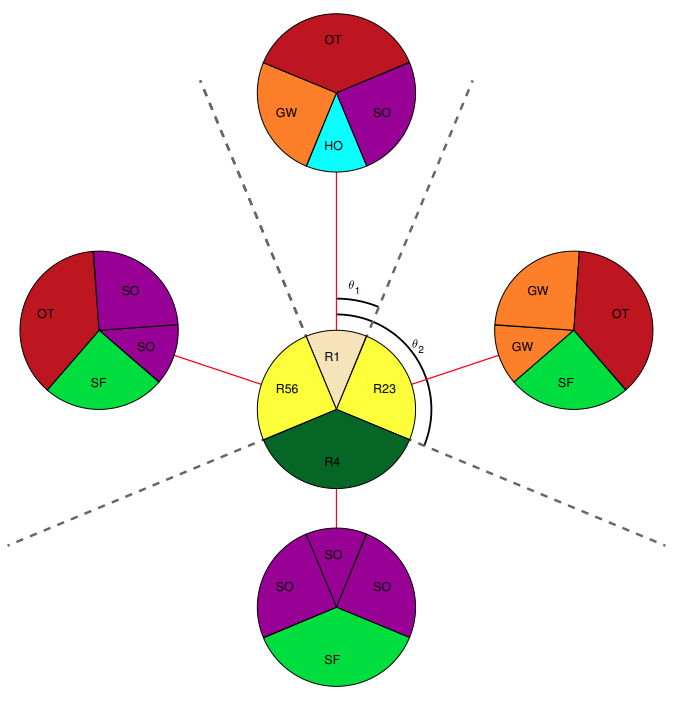
\includegraphics[height=0.35\textheight]{Images/COLREGs_assess.png}
    \caption{(TODO:ENDRE)Assigning COLREGS flag: with OS in the center we can place the TS in one of four regions. Similarly the relative bearing from TS to OS can be assigned regions with region 1 pointed directly at the OS and the rest following in a clockwise rotation.
    Courtesy of Emil Thyri.}
\end{figure}

\begin{figure}
    \centering
    \label{FIG: ship CPA}
    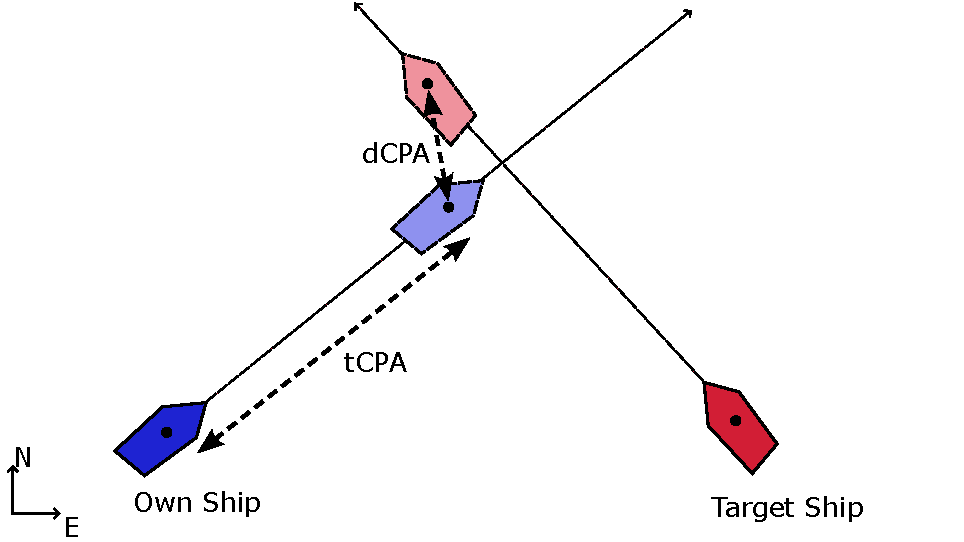
\includegraphics[width=\textwidth]{Images/shipCPA.pdf}
    \caption{Visualizing dCPA and tCPA.}
\end{figure}

\subsection{'The complete system'}
\begin{itemize}
    \item Vet ikke helt om dette kapittelet er nødvendig, men jeg lurer på om det er en god ide å skrive litt om nøyaktig hvor i ett fult funksjonelt
    system jeg forventer at min algoritme passer inn. Hva de andre delene jeg ikke kommer til å skrive om har ansvar for, og hva som forventes av systemene
    rundt mitt eget.
    \item Hvis systemet mitt var en sort boks, hvilke inputs og outputs ville det hatt.
\end{itemize}

\subsection{Simulator setup}
\begin{itemize}
    \item liten forklaring av hvordan simulatoren funker selv om jeg ikke har laget den.
    \item f.eks agent structs kan bli viktig.
    \item Forklar at det er en liten forsjel på hvordan own ship agenten og andre agenter oppdateres, fører til en maksimal 'feil' på 1 meter.
\end{itemize}



\newpage